\chapter{Vektorisasi Kata dan Dokumen}
brief of conclusion

\section{Lusia Violita Aprilian-1164080}

\subsection{Teori}

\begin{enumerate}

\item Jelaskan kenapa kata-kata harus di lakukan vektorisasi. dilengkapi dengan ilustrasi atau gambar.
	\begin{itemize}
	\item Jawaban :
		\par Kata-kata harus dilakukan vektorisasi karena kita dapat mengetahui kemiripan kata satu sama lain untuk mendapatkan kinerja yang lebih baik di mesin learning.
	\item Ilustrasi :
		\par Maksud dari kalimat di atas adalah  apabila sebelumnya menggunakan bag of word atau kantong kata yang dimana model tersebut hanya menghitung setiap kata muncul disetiap dokumen, maka disini akan menggunakan vektorisasi kata. Misal kita memiliki 2 bag of word vektor yang bisa dikatakan mirip, lalu kita dapat membandingngkan dokumen untuk melihat kemiripannya atau membandingkan kata-kata yang digunakan di kedua dokumen tersebut. Dengan kata lain, jika kedua dokumen memiliki banyak kata yang mirip dan muncul beberapa kali, mereka akan dianggap serupa.  Oleh karena itu pentingnya vektorisasi didasarkan untuk mengetahui seberapa mirip kata satu sama lain. Gambar \ref{5a1} merupakan gambaran ilustrasi.
		\begin{figure}[!hbtp]
		\centering
		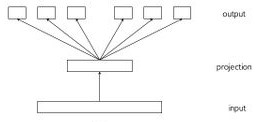
\includegraphics[scale=0.5]{figures/p1.jpg}
		\caption{Lusia-Vektorisasi}
		\label{5a1}
		\end{figure}
	\end{itemize}

\item Jelaskan mengapa dimensi dari vektor dataset google bisa sampai 300, dilengkapi
dengan ilustrasi atau gambar.
	\begin{itemize}
	\item Jawaban :
		\par Karena Google menggunakan model Word2Vec (model vektorisasi) dan setiap kata merupakan vektor yang bernilai 300 dimensi. Model yang digunakan google telah dilatih memerikas jutaan atau milyaran halaman teks. Dengan begitu google dapat menyediakan informasi yang dibutuhkan berdasarkan inputan kata kunci yang divektorisasi.
	\item Ilustrasi :
		\par Misalnya saja kita menggunakan kata kucing, anjing, dan spatula :
	
	\begin{itemize}
	\item Kucing = [0.012, 0.204, ..., -0.275, 0.056] (300 dimensi)
	\item Anjing = [0.051, -0.022, ..., -0.355, 0.227]
	\item Spatula = [ -0.191, -0.043, ..., -0.348, 0.398]
	\end{itemize}
	
	\par Persamaan terebut menjelaskan nilai dimensi dari setiap kata. Lalu dari dimensi kata tersebut kemudian dicari kesamaannya atau jaraknya, seperti berikut :	
	
	\begin{itemize}
	\item Kesamaan (jarak) antara kucing dan anjing = 0,761. Perhitungan pada gambar \ref{5a2}
		\begin{figure}[!hbtp]
		\centering
		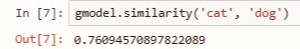
\includegraphics[scale=0.5]{figures/p2a.jpg}
		\caption{Lusia-Kesamaan Kucing Anjing}
		\label{5a2}
		\end{figure}
	\item Kesamaan antara kucing dan spatula = 0,124. Perhitungan pada gambar  \ref{5a3}
		\begin{figure}[!hbtp]
		\centering
		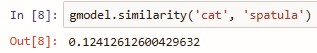
\includegraphics[scale=0.5]{figures/p2b.jpg}
		\caption{Lusia-Kesamaan Kucing Spatula}
		\label{5a3}
		\end{figure}
	\end{itemize}
	
		\par Karena hasil dari kucing dan anjing lebih tinggi maka bisa dikatakan  mirip. Maka dari itu, ketika kita mencari dengan kata kunci kucing di google, google kadang juga menyuguhkan gambar anjing karena dinilai sama.
	\end{itemize}

\item Jelaskan konsep vektorisasi untuk kata, dilengkapi dengan ilustrasi atau gambar.
	\begin{itemize}
	\item Jawaban :
		\par Konsep vektorisasi untuk kata adalah dengan mengetahui nilai dimensi dari setiap satuan kata. Lalu menghitung nilai kesamaan dimensi tersebut, setalah itu dibandingkan (seperti ilustrasi soal no.2). Vektorisasi kata (Word2Vec) menggunakan neural networks untuk mempelajari kata. Pada tingkatan kesulitan yang tinggi, neural networks mirip dengan random forest atau decission tree dan teknik machine learning lainnya karena mereka diberikan banyak input dan banyak output, sehingga dapat belajar bagaimana memprediksi output dari input. Untuk Word2Vec, input adalah satu kata dan hasilnya adalah kata-kata terdekat dari teks. Dengan demikian, Word2Vec belajar vektor kata dengan mengingat kata konteksnya.
	\item Ilustrasi :
		\par Jadi dari pemaparan soal no.2, anjing dan kucing akan memiliki vektor kata yang sama karena kedua kata ini digunakan dengan cara yang sama. Seperti contoh pada kalimat 'dia memelihara anjing' dan 'dia memelihara kucing'. Apabila 2 kalimat tersebut menggunakan model kantong kata kontinu (salah satu teknik yang digunakan untuk Word2Vec) dengan neutral networking yang mempelajari 300-dimensi perkata maka akan diperoleh hasil output yang sama. Gambar \ref{5a4} merupakan gambar ilustrasinya.
			\begin{figure}[!hbtp]
			\centering
			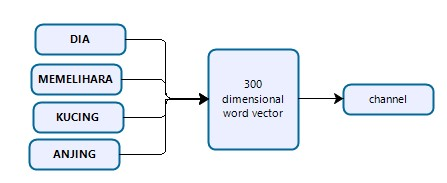
\includegraphics[scale=0.5]{figures/p3.jpg}
			\caption{Lusia-Konsep Vektorisasi Kata}
			\label{5a4}
			\end{figure}
	\end{itemize}

\item Jelaskan konsep vektorisasi untuk dokumen, dilengkapi dengan ilustrasi atau
gambar.
	\begin{itemize}
	\item Jawaban :
		\par Konsep vektorisasi dokumen mirip dengankonsep vektorisasi kata, hanya saja yang membedakan dalam hal ini inputnya adalah nama dokumen (seperti nama file) dan outputnya adalah kata-kata dari dokumen. Dan bentuk atau model yang digunakan adalah Doc2Vec.
		\par Dalam hal ini, sebagai vektor yang membantu kita memprediksi kata-kata, dari mengetahui nama file. Sebenarnya, inputnya tidak terlalu penting, yang terpenting adalah nama dari file dokumen tersebut. Kita hanya perlu melacak kata-kata yang semuanya berasal dari dokumen yang sama. Sehingga semua kata-kata akan terhubung pada nama file tersebut. Sebab itu kita dapat memprediksi kata-kata dokumen berdasarkan nama filenya, kita dapat secara efektif memiliki model yang tahu kata-kata mana yang cocok dalam sebuah dokumen. 
	\item Ilustrasi :
		\par Misalnya saja pada sebuah dokumen yang berisi ulasan atau komentar. Sebuah komentar tentunya memiliki 2 sisi yang berlawanan yaitu positif dan negatif. Dengan menggunakan vektorisasi dokumen, kita dapat mengetahui banyak kata positif yang berbeda digunakan dalam ulasan positif dan banyak kata negatif digunakan dalam ulasan negatif. Gambar \ref{5a5} merupakan gambar ilustrasinya.
			\begin{figure}[!hbtp]
			\centering
			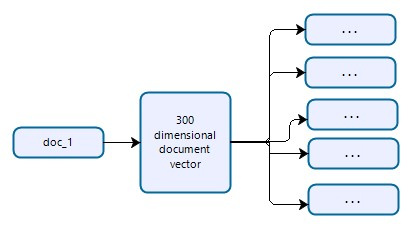
\includegraphics[scale=0.5]{figures/p4.jpg}
			\caption{Lusia-Vektorisasi Dokumen}
			\label{5a5}
			\end{figure}
	\end{itemize}

\item Jelaskan apa mean dan standar deviasi, dilengkapi dengan ilustrasi atau gambar.
	\begin{itemize}
	\item Mean
		\begin{itemize}
		\item Penjelasan :
			\par Mean atau nilai rata-rata adalah teknik penjelasan kelompok yang berdasarkan nilai rata-rat dari kelompok data.
		\item Ilustrasi :
			\par Misal kita ingin mengetahui nilai rata-rata dari suatu kelompok, maka kita bisa menjumlahkan data seluruh individu dalam kelompok tersebut. Kemudian dibagi dengan jumlah individu yang ada pada kelompok tersebut. Gambar \ref{5a6} merupakan gambar ilustrasinya.
			\begin{figure}[!hbtp]
			\centering
			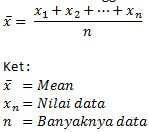
\includegraphics[scale=0.5]{figures/p5a.jpg}
			\caption{Lusia-Mean}
			\label{5a6}
			\end{figure}
		\end{itemize}
	
	\item Standar Devisiasi
		\begin{itemize}
		\item Penjelasan :
			\par Standar deviasi merupakan akar dari varians (ingat, karena pada varians kita mengkuadratkan selisih data dari rata-ratanya, maka dengan mengakarkannya, kita mendapatkan kembali nilai asalnya). Atau umumnya standar devisiasi merupakan nilai statistik yang digunakan untuk menentukan bagaimana sebaran dari data sample dan seberapa dekat titik data individu ke mean atau nilai rata-rata sample.
			
		\item Ilustrasi :
			\par Misal kita ingin mengetahui besar nilai sampel terhadap nilai rata-rata, maka kita dapat menggunakan standar deviasi. Gambar \ref{5a7} merupakan gambar ilustrasinya.
			\begin{figure}[!hbtp]
			\centering
			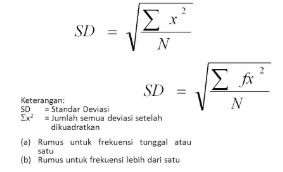
\includegraphics[scale=0.5]{figures/p5b.jpg}
			\caption{Lusia-Standar Deviasi}
			\label{5a7}
			\end{figure}
		\end{itemize}
		
	\end{itemize}

\item Jelaskan apa itu skip-gram, dilengkapi dengan ilustrasi atau gambar.
	\begin{itemize}
	\item Jawaban :
		\par Skip-gram adalah teknik pada vektorisasi kata. Skrip-gram merupakan kebalikan dari teknik kantung kata kontinus. Dimana pada teknik ini, kata tengah adalah input dan kata-kata konteks adalah output. Dalam teknik ini, vektor kata tengah digunakan untuk memprediksi kata konteks yang diberikan. 

	\item Ilustrasi :
		\par Misalkan saja kita ingin memprediksi kata, pada teknik ini vektor kata tengah digunakan untuk memprediksi kata konteks yang diberikan kata tengah. Seperti gambar \ref{5a8} : 
			\begin{figure}[!hbtp]
			\centering
			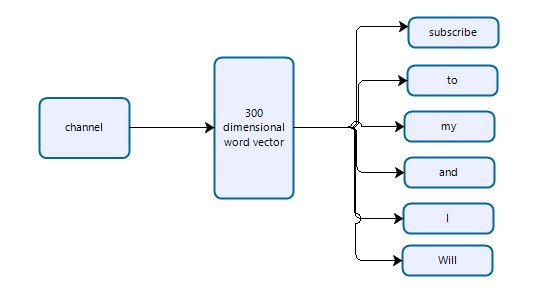
\includegraphics[scale=0.5]{figures/p6.jpg}
			\caption{Lusia-Skip gram}
			\label{5a8}
			\end{figure}
	
	\end{itemize}

\end{enumerate}

\subsection{Praktek Program}
\begin{enumerate}
\item Cobalah dataset google, dan jelaskan vektor dari kata love, faith, fall, sick, clear, shine, bag, car, wash, motor, cycle dan cobalah untuk melakukan perbandingan similirati dari masing-masing kata tersebut. jelaskan arti dari outputan similaritas dan setiap baris kode yang dibuat.
	\par Jawaban :
	\begin{enumerate}
		\item Mencoba dataset
		
			\begin{figure}[!hbtp]
			\centering
			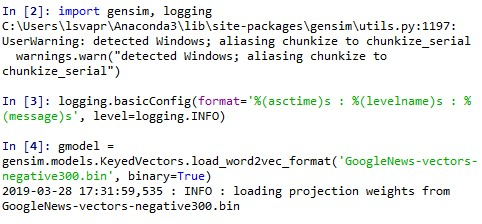
\includegraphics[scale=0.4]{figures/chap5.jpg}
			\caption{Lusia-Mencoba dataset}
			\label{5b1}
			\end{figure}
			
			\par Penjelasan gambar \ref{5b1} :
			\begin{itemize}
				\item Pada In [2] berfungsi untuk mengimport gensim untuk doc2vec dan tagging untuk opsi informasi
				\item Pada In [3] berfungsi  untuk men-setting setiap aktifitas keluar logging nya yang berisi informasi waktu, level, dan pesan.
				\item Pada In [4] berfungsi  untuk instalasi word2vec dari google model 
			\end{itemize}
			
		\item Menjelaskan vektor
			\begin{itemize}
				\item Love
					\begin{figure}[!hbtp]
					\centering
					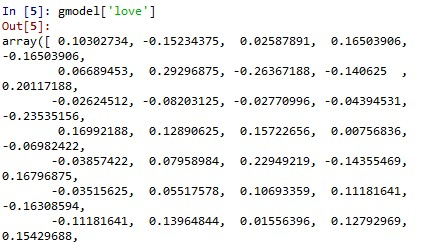
\includegraphics[scale=0.45]{figures/chap5a.jpg}
					\caption{Lusia-Menjelaskan Vektor Love}
					\label{5b2}
					\end{figure}
					\par Pada gambar \ref{5b2}, gmodel['love'] berfungsi untuk testing model love dari google model. Dan outputnya adalah berupa array. 
					
				\item Faith
					\begin{figure}[!hbtp]
					\centering
					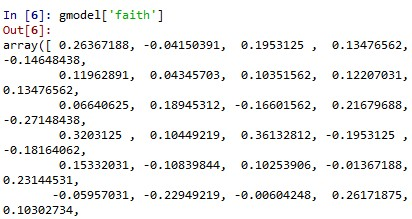
\includegraphics[scale=0.45]{figures/chap5b.jpg}
					\caption{Lusia-Menjelaskan Vektor Faith}
					\label{5b3}
					\end{figure}
					\par Pada gambar \ref{5b3}, gmodel['faith'] berfungsi untuk testing faith dari google model. Dan outputnya adalah berupa array. 
					
				\item Fall
				\begin{figure}[!hbtp]
					\centering
					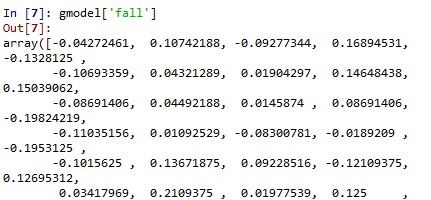
\includegraphics[scale=0.39]{figures/chap5c.jpg}
					\caption{Lusia-Menjelaskan Vektor Fall}
					\label{5b4}
					\end{figure}
					\par Pada gambar \ref{5b4}, gmodel['fall'] berfungsi untuk testing fall dari google model. Dan outputnya adalah berupa array. 
					
				\item Sick
					\begin{figure}[!hbtp]
					\centering
					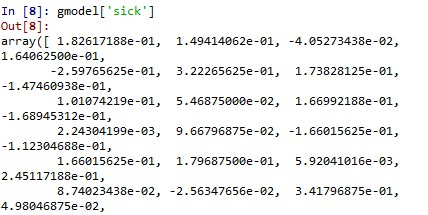
\includegraphics[scale=0.37]{figures/chap5d.jpg}
					\caption{Lusia-Menjelaskan Vektor Sick}
					\label{5b5}
					\end{figure}
					\par Pada gambar \ref{5b5}, gmodel['sick'] berfungsi untuk testing sick dari google model. Dan outputnya adalah berupa array. 
					
				\item Clear
					\begin{figure}[!hbtp]
					\centering
					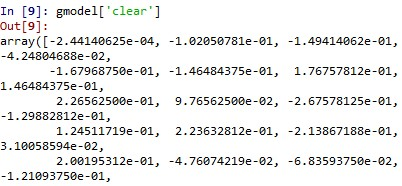
\includegraphics[scale=0.4]{figures/chap5e.jpg}
					\caption{Lusia-Menjelaskan Vektor Clear}
					\label{5b6}
					\end{figure}
					\par Pada gambar \ref{5b6}, gmodel['clear'] berfungsi untuk testing clear dari google model. Dan outputnya adalah berupa array. 
					
				\item Shine
					\begin{figure}[!hbtp]
					\centering
					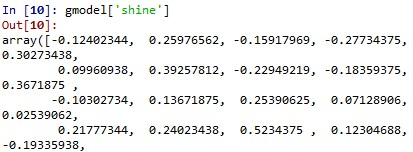
\includegraphics[scale=0.4]{figures/chap5f.jpg}
					\caption{Lusia-Menjelaskan Vektor Shine}
					\label{5b7}
					\end{figure}
					\par Pada gambar \ref{5b7}, gmodel['shine'] berfungsi untuk testing shine dari google model. Dan outputnya adalah berupa array. 
					
				\item Bag
					\begin{figure}[!hbtp]
					\centering
					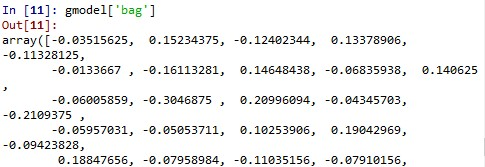
\includegraphics[scale=0.45]{figures/chap5g.jpg}
					\caption{Lusia-Menjelaskan Vektor Bag}
					\label{5b8}
					\end{figure}
					\par Pada gambar \ref{5b8}, gmodel['bag'] berfungsi untuk testing bag dari google model. Dan outputnya adalah berupa array. 
					
				\item Car
					\begin{figure}[!hbtp]
					\centering
					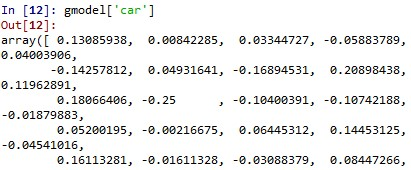
\includegraphics[scale=0.45]{figures/chap5h.jpg}
					\caption{Lusia-Menjelaskan Vektor Car}
					\label{5b9}
					\end{figure}
					\par Pada gambar \ref{5b9}, gmodel['car'] berfungsi untuk testing car dari google model. Dan outputnya adalah berupa array. 
					
				\item Wash
					\begin{figure}[!hbtp]
					\centering
					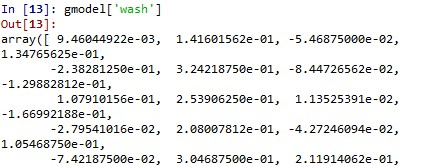
\includegraphics[scale=0.45]{figures/chap5i.jpg}
					\caption{Lusia-Menjelaskan Vektor Wash}
					\label{5b10}
					\end{figure}
					\par Pada gambar \ref{5b10}, gmodel['wash'] berfungsi untuk testing wash dari google model. Dan outputnya adalah berupa array. 
					
				\item Motor
					\begin{figure}[!hbtp]
					\centering
					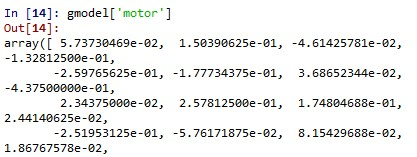
\includegraphics[scale=0.45]{figures/chap5j.jpg}
					\caption{Lusia-Menjelaskan Vektor Motor}
					\label{5b11}
					\end{figure}
					\par Pada gambar \ref{5b11}, gmodel['motor'] berfungsi untuk testing motor dari google model. Dan outputnya adalah berupa array. 
					
				\item Cycle
					\begin{figure}[!hbtp]
					\centering
					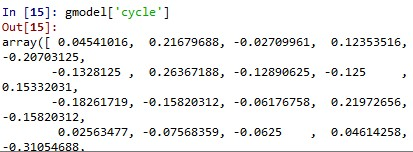
\includegraphics[scale=0.45]{figures/chap5k.jpg}
					\caption{Lusia-Menjelaskan Vektor Cycle}
					\label{5b12}
					\end{figure}
					\par Pada gambar \ref{5b12}, gmodel['cycle'] berfungsi untuk testing cycle dari google model. Dan outputnya adalah berupa array. 
			\end{itemize}
			
		\item Perbandingan similirati
			\par Dari percobaan model google, selanjutnya dibandingkan similiratinya seperti gambar \ref{5b13} berikut : 
			
			\begin{figure}[!hbtp]
			\centering
			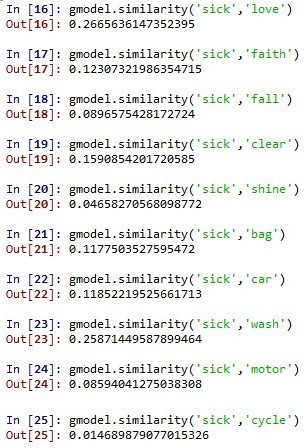
\includegraphics[scale=0.5]{figures/q1.jpg}
			\caption{Lusia-Perbandingan}
			\label{5b13}
			\end{figure}
			
			\par Penjelasan gambar \ref{5b13} 'Lusia-Perbandingan' : 
			\begin{itemize}
				\item gmodel.similarity('sick','love') untuk menecek similaritas sick dengan love dan hasilnya 0,266
				\item gmodel.similarity('sick','faith') untuk menecek similaritas sick dengan faith dan hasilnya 0,123
				\item gmodel.similarity('sick','fall') untuk menecek similaritas sick dengan fall dan hasilnya 0,089
				\item gmodel.similarity('sick','clear') untuk menecek similaritas sick dengan clear dan hasilnya 0,159
				\item gmodel.similarity('sick','shine') untuk menecek similaritas sick dengan shine dan hasilnya 0,046
				\item gmodel.similarity('sick','bag') untuk menecek similaritas sick dengan bag dan hasilnya 0,117
				\item gmodel.similarity('sick','car') untuk menecek similaritas sick dengan car dan hasilnya 0,118
				\item gmodel.similarity('sick','wash') untuk menecek similaritas sick dengan wash dan hasilnya 0.258
				\item gmodel.similarity('sick','motor') untuk menecek similaritas sick dengan motor dan hasilnya 0,085
				\item gmodel.similarity('sick','cycle') untuk menecek similaritas sick dengan cycle dan hasilnya 0,014
			\end{itemize}
			
			\par Dari hasil percobaan tersebut diperoleh nilai tertinggi 0,266. Maka yang dianggap dalam kategori kata yang sama atau mirip dengan kata sick adalah kata love.
	\end{enumerate}

\item Jelaskan dengan kata dan ilustrasi fungsi dari extract words dan PermuteSentences. 
	\begin{itemize}
		\item extract words 
			\begin{figure}[!hbtp]
			\centering
			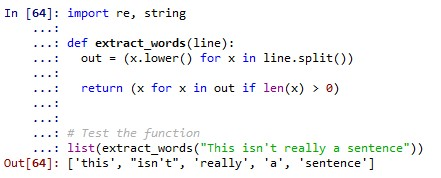
\includegraphics[scale=0.5]{figures/q2a.jpg}
			\caption{Lusia-extract words}
			\label{5b14}
			\end{figure}
			\par Penjelasan gambar \ref{5b14} : 
			\begin{itemize}
				\item Penjelasan \ref{5b14} : 
					\par Gambar 'Lusia-extract words' menjelaskan fungsi extract words. Fungsi extract words berfungsi untuk mengambil suatu argumen dengan tipe data string. Atau lebih jelasnya mengekstrak kata dari string, menghapus tanda baca, dan memisahkan kata-kata kedalam daftar.
				\item Ilustrasi \ref{5b14} : 
					\par Gambar 'Lusia-extract words' mengilustrasikan sebuah kalimat 'This isn't really a sentence' yang  akan dipisahkan perkata. Dimana library re (regex module) dan library string di import terlebih dahulu. Lalu variable out mendefinisikan X untuk mengembalikan string pada objek line yang telah di split (dibagi atau dipisahkan). Kemudian, X dikembalikan (return) berdasarkan jumlah kata. Dimana jumlah kata harus lebih dari 0. Sehingga didapat hasil output seperti pada gambar.
			\end{itemize}
			
			
		\item Permute Sentences
			\begin{figure}[!hbtp]
			\centering
			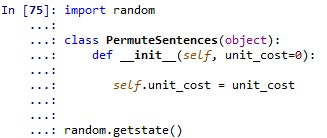
\includegraphics[scale=0.5]{figures/q2b.jpg}
			\caption{Lusia-Permute Sentences}
			\label{5b15}
			\end{figure}
			
			\par Penjelasan gambar \ref{5b15} : 
			\begin{itemize}
				\item Penjelasan \ref{5b15} : 
					\par Permute sentences berfungsi untuk melakukan random teks atau pengocokan pada sebuah teks.
				\item Ilustrasi \ref{5b15} : 
					\par Gambar 'Lusia-Permute Sentences' mengilustrasikan atribut unit cost yang akan dirandom pada sebuah class. Kemudian atribut diinisialisasi menggunakan method def init, yang dimana atribut bernilai samadengan 0. Setelah itu atribut dipresentasikan oleh 'self'. Dan yang terakhir perintah random akan mengeksekusi, sehingga menghasilkan hasil seperti gambar \ref{5b16} : 
					\begin{figure}[!hbtp]
					\centering
					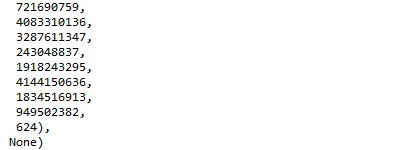
\includegraphics[scale=0.5]{figures/q2bb.jpg}
					\caption{Lusia-Hasil Permute Sentences}
					\label{5b16}
					\end{figure}
			\end{itemize}
			
	\end{itemize}

\item Jelaskan fungsi dari librari gensim TaggedDocument dan Doc2Vec disertai praktek pemakaiannya. Tunjukkan keluarannya dari komputer sendiri dan artikan maksud setiap luaran yang didapatkan.

	\begin{figure}[!hbtp]
	\centering
	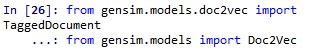
\includegraphics[scale=0.5]{figures/q3.jpg}
	\caption{Lusia-TaggedDocument dan Doc2Vec}
	\label{5b17}
	\end{figure}

	\begin{enumerate}
	\item Penjelasan fungsi :
		\par Doc2Vec telah disediakan oleh library gensim dan library tersebut memiliki sebuah class yang disebut TaggedDocument. Jadi fungsi TaggedDocument berfungsi untuk mempresentasikan kata pada dokumen dan Doc2Vec adalah model yang digunakan.
		
	\item Praktek pemakaian :
	 \par Perhatikan gambar \ref{5b17}. Gambar tersebut merupakan output dari praktek pemakaian TaggedDocument dan Doc2Vec.
	 \begin{itemize}
	 \item Baris 1 = mengimport TaggedDocument dari library gensim
	 \item Baris 2 = mengimport Doc2Vec dari library gensim
	 \end{itemize}
	  		
	\end{enumerate}

\item Jelaskan dengan kata dan praktek cara menambahkan data training dari file yang dimasukkan kedalam variabel.
	\par Perhatikan gambar \ref{5b18}.
	\begin{figure}[!hbtp]
	\centering
	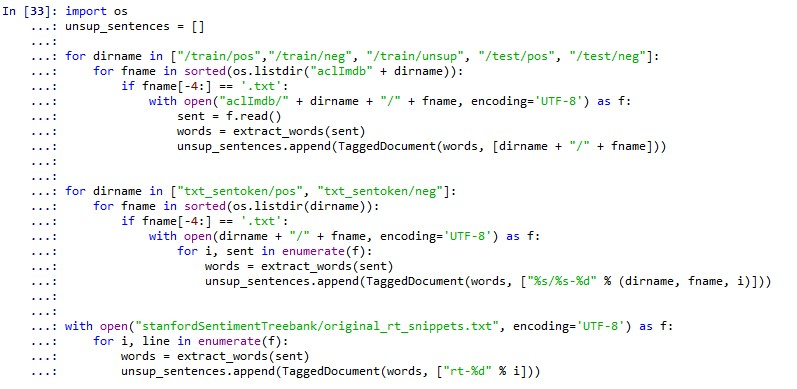
\includegraphics[scale=0.5]{figures/q4.jpg}
	\caption{Lusia-menambahkan data training}
	\label{5b18}
	\end{figure}
	\par Berikut adalah praktek cara menambahkan data training dari file yang dimasukkan kedalam variabel beserta penjelasan katanya, berdasarkan gambar \ref{5b18} :
	\begin{enumerate}
	\item Import library os
	\item membuat variable unsup sentences
	\item Berikutnya memamnggil direktori yang akan digunakan.
	\item Lalu fname memberikan nama pada direktori yang telah dipanggil.
	\item Direktori yang telah dinamai kemudian memanggil data yang bertipe data .txt.
	\item Lalu data tersebut dibuka dan di urutkan sesuai dengan list dir dengan parameter dirnamenya.
	\item Setiap data training direalisasikan pada sebuah inputan variabel words dengan extract word.
	\item Yang selanjutnya dihubungkan dengan unsup sentences yang mengeksekusi class tagged document.
	\item Dan data selesai ditambahkan.
	\end{enumerate}

\item Jelaskan dengan kata dan praktek kenapa harus dilakukan pengocokan dan pembersihan data. Tunjukkan keluarannya dari komputer sendiri dan artikan maksud setiap luaran yang didapatkan.
	\par Data harus dilakukan pengocokan supaya hasil keluaran acak tidak berurutan.  Begitu juga dilakukan pembersihan data bertujuan untuk pengecekan serta pemulihan data. Perhatikan gambar \ref{5b19}.
	\begin{figure}[!hbtp]
	\centering
	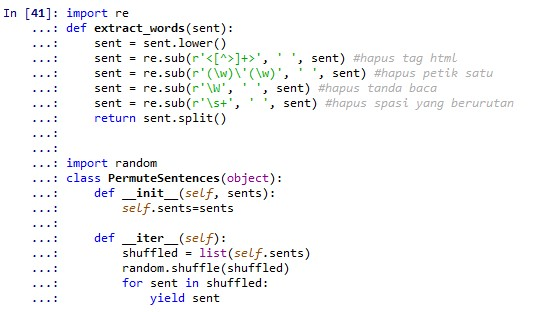
\includegraphics[scale=0.5]{figures/q5.jpg}
	\caption{Lusia-Pengocokan dan Pembersihan Data}
	\label{5b19}
	\end{figure}
	\par Gambar \ref{5b19} merupakan gambar praktik dari pengocokan dan pembersihan data. Pembersihan data dimulai dari import library re. Baris kedua penggunaan extract word dengan object sent. Baris ketiga variable sent menggunakan method lower untuk mengembalikan salinan string. Baris keempat untuk menghapus tag html, baris kelima untuk menghapus tanda baca petik satu, baris ke enam untuk menghapus tanda baca, baris ke tujuh untuk menghapus spasi yang berurutan, Dan yang teraknir untuk mengembalikan varible sent yang telah dibagi.
	\par Dan untuk pengocokan dimulai dari import library random. Lalu membuat class permute sentences yang berisi opject yang menfinisikan metode pengocokan.

\item Jelaskan dengan kata dan praktek kenapa model harus di save dan kenapa temporari training harus dihapus.Tunjukkan keluarannya dari komputer sendiri dan artikan maksud setiap luaran yang didapatkan.
	\begin{itemize}
	\item Penjelasan :
	\begin{itemize}
		\item Model harus di save karena berfungsi menyimpan data inferensi untuk mengikat vektor dokumen baru.
		\item Temporari training harus dihapus karena untuk mengosongkan sebagian memory yang telah digunakan saat melakukan training.
	\end{itemize}	  
	
	\item Praktek :
		\item Save
			\begin{figure}[!hbtp]
			\centering
			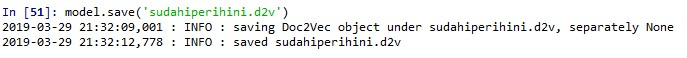
\includegraphics[scale=0.5]{figures/q6a.jpg}
			\caption{Lusia-Save}
			\label{5b20}
			\end{figure}
			
			\par Penjelasan Gambar \ref{5b20} :
			\par model.save berfungsi untuk menyimpan model yang telah dibuat. Dan dua baris dibawahnya memberikan informasi mengenai penyimpanan model tersebut.
			
		\item Delete Temporary
			\begin{figure}[!hbtp]
			\centering
			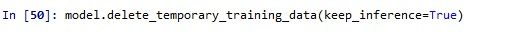
\includegraphics[scale=0.5]{figures/q6b.jpg}
			\caption{Lusia-Delete Temporary}
			\label{5b21}
			\end{figure}
			
			\par Penjelasan gambar \ref{5b21} :
			\par model.delete temporary training data berfungsi untuk menghapus beberapa data.
			
	\end{itemize}

\item jalankan dengan kata dan praktek maksud dari infer code. Tunjukkan keluarannya dari komputer sendiri dan artikan maksud setiap luaran yang didapatkan.
	\par Infer code berfungsi untuk menyimpulkan vektor yang berkaitan dengan vektor dokumen baru.
	\par Perhatikan gambar \ref{5b22}
		\begin{figure}[!hbtp]
		\centering
		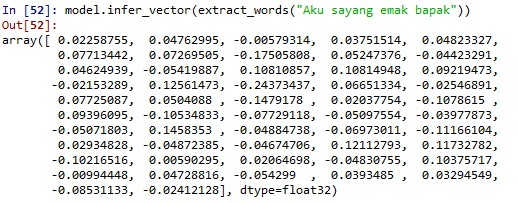
\includegraphics[scale=0.5]{figures/q7.jpg}
		\caption{Lusia-Infer code }
		\label{5b22}
		\end{figure}
	\par Gambar tersebut merupakan praktek dari infer code. Dimana infer vektor menyimpulkan vektor dari kata 'aku sayang emak bapak' yang sudah di ekstrak. Sehingga menghasilkan output berupa array dengan tipe data float32.

\item Jelaskan dengan praktek dan kata maksud dari cosine similarity. Tunjukkan keluarannya dari komputer sendiri dan artikan maksud setiap luaran yang didapatkan.
	\par Cosine similarity digunakan untuk mengecek kemiripan dari 2 kalimat berbeda. Perhatikan gambar \ref{5b23} untuk praktiknya.
		\begin{figure}[!hbtp]
		\centering
		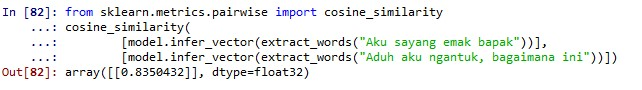
\includegraphics[scale=0.5]{figures/q8.jpg}
		\caption{Lusia-cosine similarity}
		\label{5b23}
		\end{figure}
	\par Mula-mula import cosine similarity dari library sklearn. Lalu cek kemiripan menggunakan cosine similarity yang didalamnya sudah terdapat 2 kalimat  yang akan dibandingkan. Praktek ini menggunakan kalimat 'Aku sayang emak bapak' dan kalimat 'Aduh aku ngantuk, bagaimana ini' yang menghasilkan output berupa array dengan tipe data float32.

\item Jelaskan dengan praktek score dari cross validation masing-masing metode. Tunjukkan keluarannya dari komputer sendiri dan artikan maksud setiap luaran yang didapatkan.
	\par Score dari cross validation berfungsi untuk memprediksi model yang telah dibuat dan memperkirakan keakuratannya. Perhatikan gambar \ref{5b24}
	 	\begin{figure}[!hbtp]
		\centering
		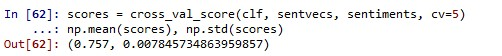
\includegraphics[scale=0.5]{figures/q9.jpg}
		\caption{Lusia-score}
		\label{5b24}
		\end{figure}
	\par Gambar \ref{5b24} merupakan praktik dari score. Gambar tersebut menjelaskan variable score yang akan menghitung keakurasian menggunakan teknik cross validation. Baris kedua merupakan perintah untuk menghitung variable score. Sehingga menghasilkan output 0.757 (akurasi = 76 persen)
\end{enumerate}

\subsection{Penanganan Error}
\begin{enumerate}
\item Skrinsut Error
	\begin{figure}[!hbtp]
	\centering
	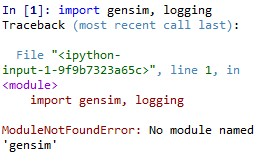
\includegraphics[scale=0.5]{figures/r1.jpg}
	\caption{Lusia-Error}
	\label{3c1}
	\end{figure}
	
\item Kode error dan jenis error
	\begin{itemize}
		\item Kode error : ModuleNotFoundError: No module named 'gensim'
		\item Jenis error : Module Not Found Error
	\end{itemize}
	
\item Solusi Pemecahan 
	\par Solusi dari permasalahan error pada skrinsut error adalah dengan mengintal modul gensim di anaconda dengan cara berikut :
	\begin{figure}[!hbtp]
	\centering
	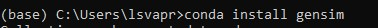
\includegraphics[scale=0.5]{figures/r3.jpg}
	\caption{Lusia-Solusi}
	\label{5c2}
	\end{figure}
\end{enumerate}















\section{Rahmi Roza-1164085}
\subsection{Teori}
Praktek Tugas Harian 
\begin{enumerate}

\item Mengapa Kata-Kata Harus di Vektorisasi
\par Kata harus di vektorisasi dikarenakan mesin hanya mampu membaca data dalam bentuk angka. Oleh karena itu diperlukan vektorisasi kata agar mesin mampu membaca data yang telah di vektorisasi. 
\par
\begin{itemize}
\item Gambar :
\par Penjelasan : Berdasarkan pengertian diatas, ada beberapa contoh yang bisa diterapkan. Untuk salah satu contoh dari klasifikasi data sendiri dapat diliat pada gambar berikut \ref{vekktorisasikataroza}.
\begin{figure}[!hbtp]
\centering
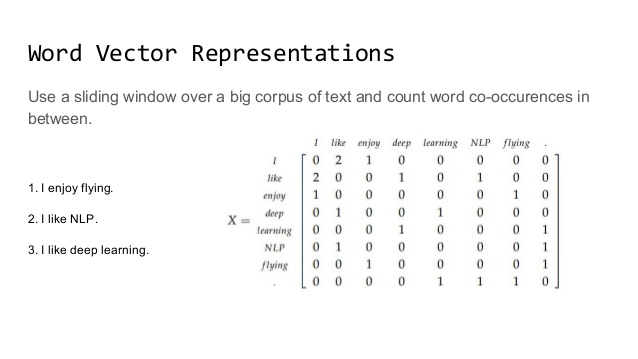
\includegraphics[scale=0.6]{figures/vekktorisasikataroza.jpg}
\caption{Vektorisasi Kata Roza}
\label{text-fadila}
\end{figure}
\end{itemize}

\item Mengapa Dimensi Dari Vektor Dataset Google Bisa Sampai 300
\par Masing-masing nilai dalam vektor 300 dimensi yang terkait dalam sebua kata "dioptimalkan" dalam  beberapa hal untuk menangkap aspek yang  berbeda dari makna dan penggunaan kata itu.Dengan kata lain masing-masing dari 300 nilai sesuai dengan beberapa fitur abstrak kata. Menghapus kombinasi nilai-nilai ini secara acak akan menghasilkan vektor yang mungkin kurang informasi penting tentang kata tersebut dan mungkin tidak lagi berfungsi sebagai representasi yang baik dari kata itu. Atau singkat cerita mungkin ada lebih dari 3 miliar kata-kata dan kalimat atau data yang tidak mungkin disimpan dalam 1 diemensi vektor makan disimpan menjadi 300 dimensi vektor untuk mengurangi kegagalan memori.
\par
\begin{itemize}
\item Gambar :
\par Penjelasan : Berdasarkan pengertian diatas, ada beberapa contoh yang bisa diterapkan. Untuk salah satu contoh dari klasifikasi data sendiri dapat diliat pada gambar berikut \ref{googleroza}.
\begin{figure}[!hbtp]
\centering
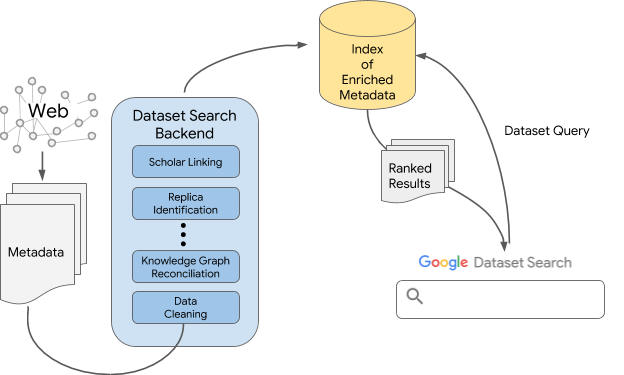
\includegraphics[scale=0.16]{figures/googleroza.png}
\caption{Google Dataset Roza}
\label{text-fadila}
\end{figure}
\end{itemize}

\item Konsep Vektorisasi Kata 
\par Konsep vektorisasi data merupakan kata-kata yang di inputkan pada mesin learning. Dan outputan nya berupa kara-kata atau keyword dari pencarian yang tekah di lakukan sebelumnya. Contoh nya pada saat kita melakukan pencarian di channel youtube kita. Maka akan muncul hasil dari pencarian dari kata-kata yang telah kita cari.
\par
\begin{itemize}
\item Gambar :
\par Penjelasan : Berdasarkan pengertian diatas, ada beberapa contoh yang bisa diterapkan. Untuk salah satu contoh dari klasifikasi data sendiri dapat diliat pada gambar berikut \ref{vekktorisasikataroza}.
\begin{figure}[!hbtp]
\centering
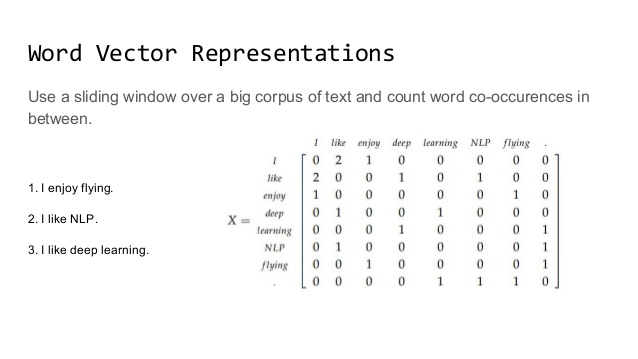
\includegraphics[scale=0.3]{figures/vekktorisasikataroza.jpg}
\caption{Vektorisasi Kata Roza}
\label{text-fadila}
\end{figure}
\end{itemize}

\item Konsep Vektorisasi Dokumen 
\par Konsep vektorisasi dokumen yaitu mesin akan membaca terlebih dahulu semua kalimat yang ada di dalam dokumen da nanti kalimat yang ada di dalam dikumen tersebut akan di oecah menjadi kata-kata.
\par
\begin{itemize}
\item Gambar :
\par Penjelasan : Berdasarkan pengertian diatas, ada beberapa contoh yang bisa diterapkan. Untuk salah satu contoh dari klasifikasi data sendiri dapat diliat pada gambar berikut \ref{vektorisasidokroza}.
\begin{figure}[!hbtp]
\centering
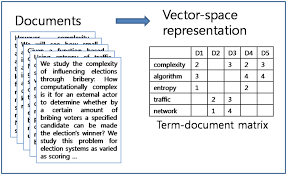
\includegraphics[scale=0.3]{figures/vektorisasidokroza.png}
\caption{Vektorisasi Dokumen Roza}
\label{text-fadila}
\end{figure}
\end{itemize}

\item Mean dan Standar Deviasi
\par Mean adalah teknik penjelasan kelompok yang didasarkan atas nilai rata-rata dari kelompok tersebut. Rata-Rata (mean) ini didapat dengan menjumlahkan data seluruh individu dalam kelompok itu, kemudian dibagi dengan jumlah individu yang ada pada kelompok tersebut. Standar deviasi adalah nilai statistik yang digunakan untuk menentukan bagaimana sebaran data dalam sampel, dan seberapa dekat titik data individu ke mean – atau rata-rata – nilai sampel.Sebuah standar deviasi dari kumpulan data sama dengan nol menunjukkan bahwa semua nilai-nilai dalam himpunan tersebut adalah sama. Sebuah nilai deviasi yang lebih besar akan memberikan makna bahwa titik data individu jauh dari nilai rata-rata.
\par
\begin{itemize}
\item Gambar :
\par Penjelasan : Berdasarkan pengertian diatas, ada beberapa contoh yang bisa diterapkan. Untuk salah satu contoh dari klasifikasi data sendiri dapat diliat pada gambar berikut \ref{meanroza}.
\begin{figure}[!hbtp]
\centering
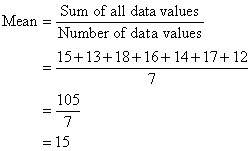
\includegraphics[scale=0.2]{figures/meanroza.png}
\caption{Mean Roza}
\label{text-fadila}
\end{figure}
\begin{figure}[!hbtp]
\centering
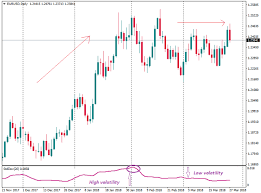
\includegraphics[scale=0.2]{figures/standarroza.png}
\caption{Standar Deviasi Roza}
\label{text-fadila}
\end{figure}
\par
\end{itemize}

\item Skip Gram
\par Skip-Gram mencoba memprediksi vektor kata-kata yang ada di konteks diberikan vektor kata tertentu. Skip-gram membuat sepasang kata target dan konteks sebagai sebuah instance sehingga skip-gram cenderung lebih baik ketika ukuran corpus sangat besar.
\par
\begin{itemize}
\item Gambar :
\par Penjelasan : Berdasarkan pengertian diatas, ada beberapa contoh yang bisa diterapkan. Untuk salah satu contoh dari klasifikasi data sendiri dapat diliat pada gambar berikut \ref{skipgramroza}.
\begin{figure}[!hbtp]
\centering
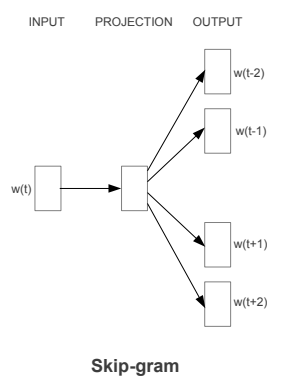
\includegraphics[scale=0.2]{figures/skipgramroza.png}
\caption{Skip-Gram Roza}
\label{text-fadila}
\end{figure}
\end{itemize}
\end{enumerate}

\begin{itemize}
\item Plagiarisme Roza
\begin{figure}[!hbtp]
\centering
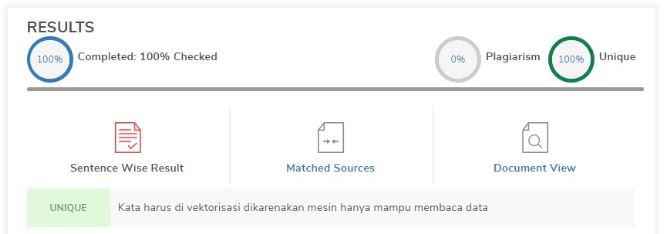
\includegraphics[scale=0.2]{figures/plagiarismeroza.jpg}
\caption{Plagiarisme Roza}
\label{text-fadila}
\end{figure}
\end{itemize}


\subsection{Praktek}
\begin{enumerate}
\item Contoh Dataset Google dan Menjelaskan Vektor  Dari Kata-Kata Yang Telah Ditentukan
\par
\begin{itemize}
\item Love
\begin{figure}[!hbtp]
\centering
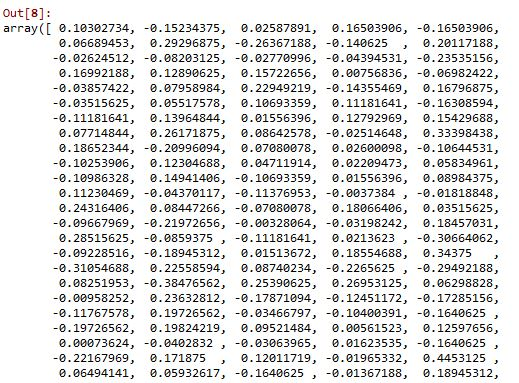
\includegraphics[scale=0.6]{figures/loveroza.jpg}
\caption{Love Roza}
\label{text-fadila}
\end{figure}
\par Penjelasan Hasil: Dapat dilihat pada hasil gambar, bahwa nilai vektor pada baris pertamanya adalah 0.10302734
\par
\item Faith
\begin{figure}[!hbtp]
\centering
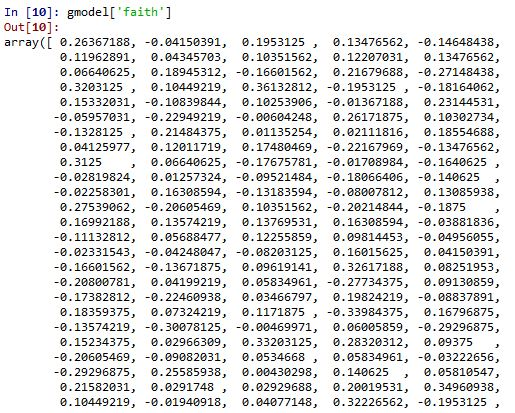
\includegraphics[scale=0.6]{figures/faithroza.jpg}
\caption{Faith Roza}
\label{text-fadila}
\end{figure}
\par Penjelasan Hasil: Pada hasil gambar faith dapat dilihat bahwa nilai pada vektor baris pertamanya adalah 0.26367188. Jika dibandingkan dengan gambar love dapat dikatakan bahwa kedua gambar tersebut dapat dimasukkan pada kategori yang sama.
\item Fall
\begin{figure}[!hbtp]
\centering
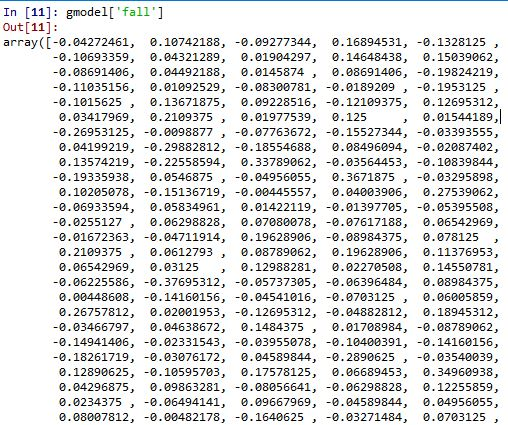
\includegraphics[scale=0.6]{figures/fallroza.jpg}
\caption{Fall Roza}
\label{text-fadila}
\end{figure}
\par Penjelasan Hasil: Pada hasil gambar fall dapat dilihat bahwa nilai pada vektor baris pertamanya adalah -0.04. Jika dibandingkan dengan gambar faith dapat dikatakan bahwa kedua gambar tersebut tidak dapat dimasukkan pada kategori yang sama.
\item Sick
\begin{figure}[!hbtp]
\centering
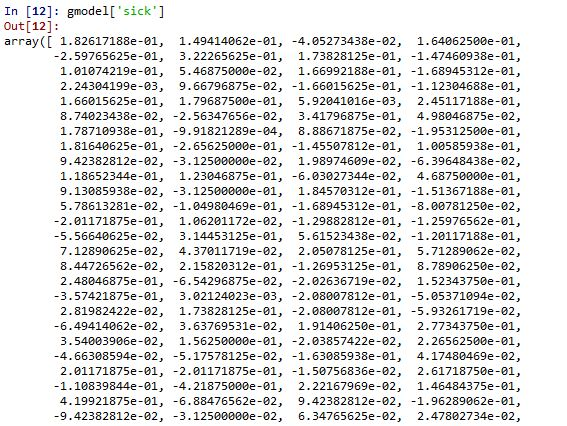
\includegraphics[scale=0.6]{figures/sickroza.jpg}
\caption{Sick Roza}
\label{text-fadila}
\end{figure}
\par Penjelasan Hasil: Pada hasil gambar sick dapat dilihat bahwa nilai pada vektor baris pertamanya adalah 1.82. Jika dibandingkan dengan gambar fall dapat dikatakan bahwa kedua gambar tersebut tidak dapat dimasukkan pada kategori yang sama.
\item Clear
\begin{figure}[!hbtp]
\centering
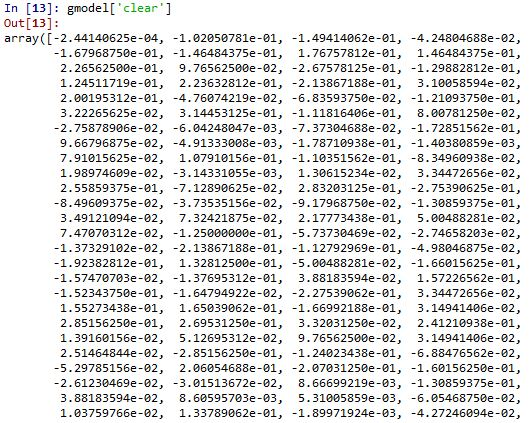
\includegraphics[scale=0.6]{figures/clearroza.jpg}
\caption{Clear Roza}
\label{text-fadila}
\end{figure}
\par Penjelasan Hasil: Pada hasil gambar clear dapat dilihat bahwa nilai pada vektor baris pertamanya adalah -2.44. Jika dibandingkan dengan gambar sick dapat dikatakan bahwa kedua gambar tersebut tidak dapat dimasukkan pada kategori yang sama.
\item Shine
\begin{figure}[!hbtp]
\centering
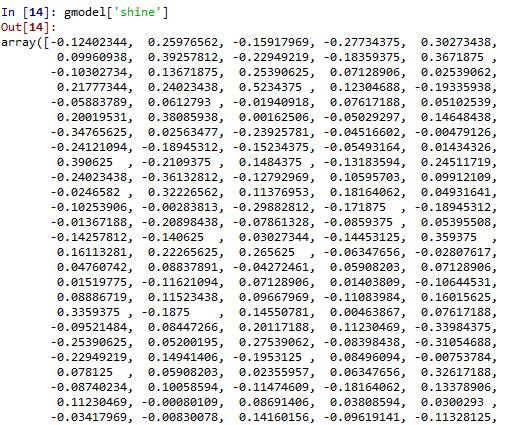
\includegraphics[scale=0.6]{figures/shineroza.jpg}
\caption{Shine Roza}
\label{text-fadila}
\end{figure}
\par Penjelasan Hasil: Pada hasil gambar shine dapat dilihat bahwa nilai pada vektor baris pertamanya adalah -0.12. Jika dibandingkan dengan gambar clear dapat dikatakan bahwa kedua gambar tersebut tidak dapat dimasukkan pada kategori yang sama.
\item Bag
\begin{figure}[!hbtp]
\centering
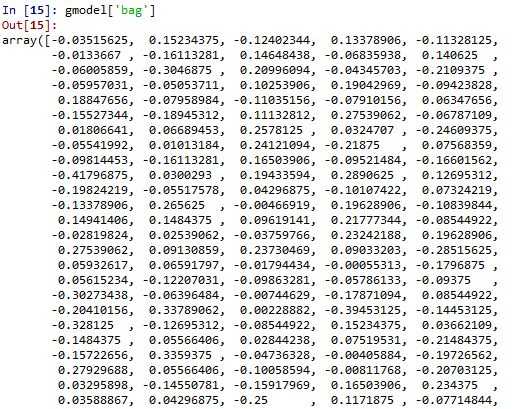
\includegraphics[scale=0.6]{figures/bagroza.jpg}
\caption{Bag Roza}
\label{text-fadila}
\end{figure}
\par Penjelasan Hasil: Pada hasil gambar bag dapat dilihat bahwa nilai pada vektor baris pertamanya adalah -0.035. Jika dibandingkan dengan gambar shine dapat dikatakan bahwa kedua gambar tersebut  dapat dimasukkan pada kategori yang sama.
\item Car
\begin{figure}[!hbtp]
\centering
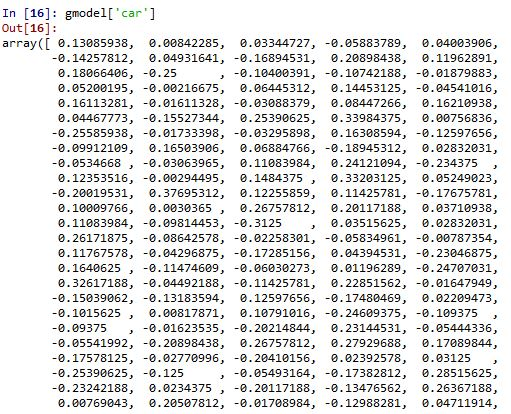
\includegraphics[scale=0.6]{figures/carroza.jpg}
\caption{Car Roza}
\label{text-fadila}
\end{figure}
\par Penjelasan Hasil: Pada hasil gambar car dapat dilihat bahwa nilai pada vektor baris pertamanya adalah -0.13. Jika dibandingkan dengan gambar bag dapat dikatakan bahwa kedua gambar tersebut  dapat dimasukkan pada kategori yang sama
\item Wash
\begin{figure}[!hbtp]
\centering
\includegraphics[scale=0.6]{figures/washroza.jpg}
\caption{Wash Roza}
\label{text-fadila}
\end{figure}
\par Penjelasan Hasil: Pada hasil gambar wash dapat dilihat bahwa nilai pada vektor baris pertamanya adalah 9.460. Jika dibandingkan dengan gambar car dapat dikatakan bahwa kedua gambar tersebut tidak dapat dimasukkan pada kategori yang sama
\item Motor
\begin{figure}[!hbtp]
\centering
\includegraphics[scale=0.6]{figures/motorroza.jpg}
\caption{Motor Roza}
\label{text-fadila}
\end{figure}
\par Penjelasan Hasil:  Pada hasil gambar motor dapat dilihat bahwa nilai pada vektor baris pertamanya adalah 5.737. Jika dibandingkan dengan gambar wash dapat dikatakan bahwa kedua gambar tersebut tidak dapat dimasukkan pada kategori yang sama.
\item Cycle
\begin{figure}[!hbtp]
\centering
\includegraphics[scale=0.6]{figures/cycleroza.jpg}
\caption{Cycle Roza}
\label{text-fadila}
\end{figure}
\par Penjelasan:  Pada hasil gambar cycle dapat dilihat bahwa nilai pada vektor baris pertamanya adalah 0.045. Jika dibandingkan dengan gambar motor dapat dikatakan bahwa kedua gambar tersebut tidak dapat dimasukkan pada kategori yang sama.


\item Perbandingan Similirati
\begin{figure}[!hbtp]
\centering
\includegraphics[scale=0.6]{figures/perbandinganrozaa.jpg}
\caption{Perbandingan Similariti Roza}
\label{text-fadila}
\end{figure}
\par Penjelasan Hasil: Pada gambar tersebut dapat dilihat bahwa perbandingan antara car dan faith tidak dapat dimasukkan pada kaegori yang sama karena memounyai nilai yang kecil. Begitu juga dengan car,clear dan car shine. Sedangkan pada car, fall dan car, sick bisa dikatakan mempunyai kategori yang sama.

\end{itemize}
\item Fungsi Dari Extract word Dan PermuteSentences
\par
\begin{itemize}
\item Extract Word
\par Penjelasan: Exstract word bergungsi untuk mengambil suatu argumen dengan type data string.
\begin{figure}[!hbtp]
\centering
\includegraphics[scale=0.6]{figures/wordroza.jpeg}
\caption{Extract Word Roza}
\label{text-fadila}
\end{figure}
\par Penjelasan Hasil:  mengilustrasikan sebuah kalimat 'Mohon maaf saya sudah mengantuk' yang  akan dipisahkan perkata. Dimana library re (regex module) dan library string di import terlebih dahulu. Lalu variable out mendefinisikan X untuk mengembalikan string pada objek line yang telah di split (dibagi atau dipisahkan). Re.sub digunakan untuk mengembalikan string yang diperoleh dengan mengganti kemunculan pola dalam string yang paling tidak tumpang tindih dengan repl pengganti. Kemudian, X dikembalikan berdasarkan jumlah kata. Sehingga didapat hasil output seperti pada gambar.


\item PermuteSentence
\par Penjelasan: PermuteSentences berfungsi untuk melakukan pengocokan atau random pada teks.
\begin{figure}[!hbtp]
\centering
\includegraphics[scale=0.6]{figures/permutesenroza.jpg}
\caption{PermueSentences Roza}
\label{text-fadila}
\end{figure}
\par Penjelasan: Pada gambar di atas dapat dikatakan bahwa dari huruf abjad tersebut dikocok atau di random secara ascenden. Dan hasilnya adalah huruf j.
\end{itemize}


\item Fungsi dari Librari Gensim TaggedDocument dan Doc2Vec
\par
\begin{itemize}
\begin{figure}[!hbtp]
\centering
\includegraphics[scale=0.6]{figures/1rozaa.jpg}
\caption{No 3 Roza}
\label{text-fadila}
\end{figure}
\item Penjelasan Hasil:  Pada baris pertama yaitu mengimport modul Tagged Document dari model gensim. Sedangkan pada baris kedua import Doc2vec dari model gensim.
\end{itemize}

\item Cara Menambahkan Data Training
\par Penskalaan yaitu dataset ditempatkan sambil mempertimbangkan kumpulan data linier seperti data bank.
\par Disintegrasi dan Komposisi: Langkah ini melibatkan pemecahan fitur tertentu untuk membangun data pelatihan yang lebih baik untuk model yang Anda pahami lebih komprehensif.
\par Komposisi: Ini adalah proses terakhir yang melibatkan penggabungan berbagai fitur menjadi satu fitur untuk mendapatkan data yang lebih akurat atau bermakna.
\begin{itemize}
\begin{figure}[!hbtp]
\centering
\includegraphics[scale=0.6]{figures/3roza.jpg}
\caption{No 4 Roza}
\label{text-fadila}
\end{figure}
\item  Penjelasan Hasil: Membaca direktori name dari data yang ada di dalam kurung. Pada kodingan di atas ada 3 data. Data pertama yaitu: train/pos,train/neg, train/unsuo, test/pos dan test/neg. Data kedua yaitu:txtsentoken/pos dan txt/sentokenneg. Sedangkan data ke 3 yaitu: standfordSentimentTreeBank/Originalrtsnippes.txt
\end{itemize}


\item Kenapa Harus Dilakukan Pengocokan dan Pembersih Data
\par Pengocokan data dilakukan untuk merandom data-data yang ada. Sedangkan pembersihan data dilakukan untuk pengecekan data untuk penetapan dan pemulihan data yang hilang, pengecekan penentapan meliputi pemerikasaan data yang out of range (di luar cakupan) tidak konsisten secara logika, ada nilai-nilai ekstrim, data dengan nilai-nilai tdk terdefinisi, sedangkan pemulihan data yang hilang adalah nilai dari suatu variabel yang tidak diketahui dikarenakan  jawaban responden yang membingungkan.
\begin{itemize}
\begin{figure}[!hbtp]
\centering
\includegraphics[scale=0.6]{figures/4broza.jpg}
\caption{No 5 Roza}
\label{text-fadila}
\end{figure}
\item Penjelasan Hasil: Pada gambar pertama yaitu melakukan pengacakan model terhadap data unsupervised learning. Dan kemudian baru membuat modelnya setelah dilakukan pengacakan terhadap yang pertama tadi.
\begin{figure}[!hbtp]
\centering
\includegraphics[scale=0.6]{figures/4roza.jpg}
\caption{No 5 Roza}
\label{text-fadila}
\end{figure}
\item Penjelasan Hasil:  Mengimport Library Re. Kemudian membuat fungsi utuk menghapus tag html dan perkocokan. Dimana di dalam variabel ini ada kodingan untuk menghapus tag html yaitu petik satu, tanda baca dan spasi yang berurutan.
\end{itemize}

\item Model harus di Save dan Kenapa Temporari Training Harus Dihapus
\par Kenapa model harus di save berfungsi untuk mencegah ram agar tidak lemot. Sedangkan kenapa temporari training harus dihapus mengosongkan memori agar sedikit lega atau tidak lemot.
\begin{itemize}
\begin{figure}[!hbtp]
\centering
\includegraphics[scale=0.6]{figures/6roza.jpeg}
\caption{No 6 Roza}
\label{text-fadila}
\end{figure}
\item Penjelasan Hasil: Menghapus Temporary Training Data
\begin{figure}[!hbtp]
\centering
\includegraphics[scale=0.6]{figures/6broza.jpeg}
\caption{No 6 Roza}
\label{text-fadila}
\end{figure}
\item Penjelasan Hasil: Menyimpan model rozroza.d2v
\end{itemize}


\item InferCode
\par Infercode digunakan untuk menyimpulkan vektor yang berhubungan dengan vektor dokumen baru.
\begin{itemize}
\begin{figure}[!hbtp]
\centering
\includegraphics[scale=0.6]{figures/7roza.jpeg}
\caption{No 7 Roza}
\label{text-fadila}
\end{figure}
\item Penjelasan Hasil:  Pada hasil gambar tersebut dapat disimpulkan bahwa kalimat "Roza LDR an Jauh Parah" menghasilkan outputan berupa array seperti angka-angka di bawah.
\end{itemize}

\item Cosine Similarity.
\par
\begin{itemize}
\begin{figure}[!hbtp]
\centering
\includegraphics[scale=0.6]{figures/8roza.jpeg}
\caption{No 8 Roza}
\label{text-fadila}
\end{figure}
\item  Penjelasan Hasil:  Pada gambar di atas yaitu mengimport cosine similartity dari sklearn metrics pairwise. Dimana cosine similarity berfungsi untuk mengecek kemiripan dari kalimat Services Sucks. Dan akan muncul hasilnya yaitu array.
\end{itemize}

\item Score Dari Cross Validation
\par
\begin{itemize} 
\begin{figure}[!hbtp]
\centering
\includegraphics[scale=0.6]{figures/9roza.jpeg}
\caption{No 9 Roza}
\label{text-fadila}
\end{figure}
\item  Penjelasan Hasil:  Menghitung model clrf, sentvecs, setiments serta juga meghitung keakuratannya.
\end{itemize}

\subsection{Penanganan Error}
\begin{enumerate}
\item Skrinsut Error
\begin{figure}[ht]
\centering
\includegraphics[scale=0.5]{figures/errorrozaaa.jpg}
\caption{ Error Roza}
\label{6}
\end{figure}
\item Kode Error dan Jenis Errornya
\par Kode Error: "NameError: name 'unsup sentences is not defined". 
\par Jenis Error: Unsup Sentence Not Defined
\item Penanganan
\par Running ulang dari awal, sehingga unsupervide baru bisa ditemukan.


\end{enumerate}
\end{enumerate}

\par
\par
\par
\par
\par
\section{Fadila-1164072}
\subsection{Teori}
Penjelasan Tugas Harian 9 ( No 1-6 ). ( No. 7 Bukti Plagiarisme )
\begin{enumerate}
\item Mengapa Kata-Kata Harus Di Lakukan Vektorisasi Dan Ilustrasi Gambar
\begin{itemize}
\item Penjelasan :
\par Alasan mengapa kata-kata harus dilakukan vektorisasi terlebih dahulu yaitu dikarenakan mesin hanya mampu membaca data dengan bentuk angka. Berdasarkan hal tersebut maka tentunya diperlukan vektorisasi kata atau bisa disebut dengan mengubah kata menjadi bentuk vektor agar mesin seolah-olah paham apa yang kita maksudkan dan dapat memproses aktifitas/perintah dengan benar. Kata juga harus di vektorisas iuntuk mengetahui presentase kata yang sering muncul dalam setiap kalimatnya, yang berguna untuk menetukan kata kunci.
\par
\item Ilustrasi Gambar
\par Penjelasan : Berdasarkan penjelasan diatas, ada beberapa contoh yang bisa diterapkan. Untuk salah satu contoh dari vektorisasi kata dapat diliat pada gambar berikut \ref{Vektorisasi Kata-fadila}.
\begin{figure}[!hbtp]
\centering
\includegraphics[scale=0.2]{figures/word-vec-fadila.jpg}
\caption{Vektorisasi Kata-fadila}
\label{Vektorisasi Kata-fadila}
\end{figure}
\par
\end{itemize}
\par
\par
\item Mengapa Dimensi Dari Vektor Dataset Google Bisa Mencapai 300 Dan Ilustrasi Serta Contoh Gambar
\begin{itemize}
\item  Penjelasan :
\par Dimensi dari Vektor Dataset Google Bisa Mencapai 300 itu dikarenakan pada masing-masing objek yang terdapat pada dataset akan memiliki identitasnya tersendiri, selain itu juga untuk nilai dalam vektor 300 dimensi yang terkait dalam sebua kata "dioptimalkan" dalam  berbagai hal untuk menangkap aspek yang berbeda dari makna dan penggunaan kata itu. secara singkatnya terdapat ada lebih dari 3 miliar kata-kata dan kalimat yang tidak mungkin disimpan dalam 1 diemensi vektor, lalu disimpan menjadi 300 dimensi vektor untuk mengatasi yang namanya kegagalan memori
\item Ilustrasi :( berdasarkan identitas tersendiri ) Apabila dicontohkan dengan penjelasan yang lebih rinci maka dilakukan perumpamaan sederhana. Misalnya untuk sebuah dataset google yang memiliki 3 buah objek yaitu berat, lebar, dan tinggi.  Kemudian dari masing-masing objek tersebut dilakukan perbandingan antara berat dan lebar beserta berat dan tinggi. Hasil yang didapatkan akan memiliki presentasi yang berbeda sehingga dapat diartikan bahwa mesin dapat membedakan objek yang hampir serupa namun tak sama.
\par 
\item Contoh Gambar
\par Penjelasan : Berdasarkan penjelasan diatas, ada beberapa contoh yang lain bisa diterapkan. Untuk salah satu contoh dari vektor dataset googlei dapat diliat pada gambar berikut \ref{Dimensi Vektor Dataset Wikipedia-fadila} dan \ref{Dimensi Vektor Dataset-fadila}.
\begin{figure}[!hbtp]
\centering
\includegraphics[scale=0.15]{figures/google-dataset-wikipedia-fadila.jpg}
\caption{Dimensi Vektor Dataset Wikipedia-fadila}
\label{Dimensi Vektor Dataset Wikipedia-fadila}
\end{figure}
\par
\begin{figure}[!hbtp]
\centering
\includegraphics[scale=0.15]{figures/google-dataset-fadila.jpg}
\caption{Dimensi Vektor Dataset -fadila}
\label{Dimensi Vektor Dataset-fadila}
\end{figure}
\par
\end{itemize}
\par
\par
\item Konsep Vektorisasi Untuk Kata Dan Ilustrasi Gambar
\begin{itemize}
\item  Penjelasan :
\par Konsep untuk vektorisasi kata sebenarnya sama dengan ketika dilakukan input suatu kata pada mesin pencarian. Kemudian untuk hasilnya akan mengeluarkan ( berupa ) referensi mengenai kata tersebut. Jadi data kata tersebut didapatkan dari hasil pengolahan pada kalimat-kalimat sebelumnya yang telah diolah. Contoh sederhananya pada kalimat berikut ( Please click the alarm icon for more notifications about my channel ), pada kalimat tersebut terdapat konteks yakni channel, kata tersebut akan dijadikan data latih untuk mesin yang akan dipelajari dan diproses. Jadi ketika kita inputkan kata channel, maka mesin akan menampilkan keterkaitannya dengan kata tersebut sehingga akan lebih efisien dan lebih mudah.
\par
\item Ilustrasi Gambar
\par Penjelasan : Berdasarkan konsep diatas, ada beberapa contoh yang bisa diterapkan. Untuk salah satu contoh dari vektorisasi kata dapat diliat pada gambar berikut \ref{Vektorisasi Untuk Kata-fadila}.
\begin{figure}[!hbtp]
\centering
\includegraphics[scale=0.2]{figures/concept-word-fadila.jpg}
\caption{Vektorisasi Untuk Kata-fadila}
\label{Vektorisasi Untuk Kata-fadila}
\end{figure}
\par
\end{itemize}
\par
\par
\item Konsep Vektorisasi Untuk Dokumen Dan Ilustrasi Gambar
\begin{itemize}
\item  Penjelasan :
\par Untuk vektorisasi dokumen sebenarnya terbilang sama dengan konsep vektorisasi kata, yang membedakan hanya pada proses awalnya ( pada eksekusi awal ). Untuk vektorisasi dokumen ini, mesin akan membaca semua kalimat yang terdapat pada dokumen tersebut, kemudian kalimat yang terdapat pada dokumen tersebut akan di pecah menjadi kata-kata. Seperti itulah konsep vektorisasi dokumen.
\par
\item Ilustrasi Gambar
\par Penjelasan : Berdasarkan konsep diatas, ada beberapa contoh yang bisa diterapkan. Untuk salah satu contoh dari vektorisasi dokumen dapat diliat pada gambar berikut \ref{Vektorisasi Untuk Dokumen-fadila}.
\begin{figure}[!hbtp]
\centering
\includegraphics[scale=0.2]{figures/doc-vec-fadila.jpg}
\caption{Vektorisasi Untuk Dokumen-fadila}
\label{Vektorisasi Untuk Dokumen-fadila}
\end{figure}
\par
\end{itemize}
\par
\par
\item Pengertian Mean Dan Standar Devisiasi Beserta Ilustrasi Gambar
\begin{itemize}
\item  Pengertian Mean :
\par Mean merupakan nilai rata-rata dari suatu data. Mean sendiri dapat dicari dengan cara membagi jumlah data dengan banyak data sehingga diperoleh lah nilai rata-rata dari suatu data yang dicari / tersebut. 
\par
\par
\item  Pengertian Standar Devisiasi :
\par Untuk standar deviasi sendiri merupakan sebuah teknik statistik yang digunakan dalam menjelaskan homogenitas kelompok ataupun dapat diartikan dengan nilai statistik dimana dimanfaatkan untuk menentukan bagaimana sebaran data dalam sampel, serta seberapa dekat titik data individu ke mean atau rata-rata nilai sampel yang ada. 
\par
\par
\item Ilustrasi Gambar
\par Penjelasan : Berdasarkan penjelasan diatas, ada beberapa contoh yang bisa diterapkan. Untuk salah satu contoh dari mean dan standar devisiasi sendiri dapat diliat pada gambar berikut \ref{Mean-fadila} , \ref{Mean2-fadila}  dan \ref{Standar Devisiasi-fadila}.
\begin{figure}[!hbtp]
\centering
\includegraphics[scale=0.17]{figures/mean-fadila.jpg}
\caption{Mean-fadila}
\label{Mean-fadila}
\end{figure}
\par
\begin{figure}[!hbtp]
\centering
\includegraphics[scale=0.17]{figures/mean2-fadila.jpg}
\caption{Mean Lanjutan-fadila}
\label{Mean2-fadila}
\end{figure}
\par
\begin{figure}[!hbtp]
\centering
\includegraphics[scale=0.17]{figures/deviasi-fadila.jpg}
\caption{Standar Devisiasi-fadila}
\label{Standar Devisiasi-fadila}
\end{figure}
\par
\end{itemize}
\par
\par
\item Penjelasan Skip-gram Dan Ilustrasi Gambar
\begin{itemize}
\item  Penjelasan :
\par Sebuah  teknik yang digunakan di area speech processing, dimana n-gram yang dibentuk kemudian ditambahkan juga dengan tindakan “skip” pada token-tokennya. 
\par Untuk membentuk k-skip-n-grams, ada dua nilai yang harus didefinisikan, dimana kedua nilai tersebut yaitu k (jumlah kata yang di-skip) dan n (banyak kata dalam n-gram, e.g. bigram (2-gram), trigram (3-gram), dll.).
\par
\item Ilustrasi Gambar
\par Penjelasan : Berdasarkan penjelasan diatas, ada beberapa contoh yang bisa diterapkan. Untuk salah satu contoh dari skip-gram sendiri dapat diliat pada gambar-gambar berikut \ref{Plagiarisme - fadila} .
\begin{figure}[!hbtp]
\centering
\includegraphics[scale=0.17]{figures/skip-gram-fadila.jpg}
\caption{Skip Gram - fadila}
\label{Skip Gram - fadila}
\end{figure}
\par
\par
\end{itemize}
\par
\par
\par
\par
\item Plagiarisme Fadila :
\begin{figure}[!hbtp]
\centering
\includegraphics[scale=0.2]{figures/plagiarismm-fadila.jpg}
\caption{Plagiarisme - fadila}
\label{Plagiarisme - fadila}
\end{figure}
\end{enumerate}
\par
\par
\par
\par
\par


\subsection{Praktek}
Penjelasan Tugas Harian 10 ( No 1-9 ). ( Dan Penanganan Error )
\begin{enumerate}
\item Percobaan Google Dataset ( Perbandingan Dan Similarity ) Untuk Beberapa Data Berikut :
\par Note : Penjelasan setiap datasetnya saya berikan perbandingan langsung untuk contoh yang lebih jelas sebelum dilakukan similarity ( dengan dataset tertentu ).
\begin{enumerate}
\item Love : Berpatokan pada gambar \ref{Google Dataset - Love - fadila}.
\par Penjelasan : Pada hasil gambar love dapat dilihat bahwa nilai pada vektor baris pertamanya yaitu sebesar -0.10.
\par
\begin{figure}[!hbtp]
\centering
\includegraphics[scale=0.3]{figures/1-love-fadila.jpg}
\caption{Google Dataset - Love - fadila}
\label{Google Dataset - Love - fadila}
\end{figure}
\par
\item Faith :  Berpatokan pada gambar \ref{Google Dataset - Faith- fadila}.
\par Penjelasan : Pada hasil gambar faith dapat dilihat bahwa nilai pada vektor baris pertamanya yaitu sebesar -0.26. Jika dibandingkan dengan gambar love dapat dikatakan bahwa kedua gambar tersebut dapat dimasukkan pada kategori yang sama dikarenakan nilainya mendekati/dekat/hampir sama.
\par
\begin{figure}[!hbtp]
\centering
\includegraphics[scale=0.3]{figures/1-faith-fadila.jpg}
\caption{Google Dataset - Faith- fadila}
\label{Google Dataset - Faith- fadila}
\end{figure}
\par
\item Fall :  Berpatokan pada gambar \ref{Google Dataset - Fall - fadila}.
\par Penjelasan : Pada hasil gambar fall dapat dilihat bahwa nilai pada vektor baris pertamanya yaitu sebesar -0.04. Jika dibandingkan dengan gambar faith dapat dikatakan bahwa kedua gambar tersebut tidak dapat dimasukkan pada kategori yang sama karena nilainya berbeda ( tidak dalam range yang dekat ).
\par
\begin{figure}[!hbtp]
\centering
\includegraphics[scale=0.3]{figures/1-fall-fadila.jpg}
\caption{Google Dataset - Fall - fadila}
\label{Google Dataset - Fall - fadila}
\end{figure}
\par
\item Sick :  Berpatokan pada gambar \ref{Google Dataset - Sick - fadila}.
\par Penjelasan : Pada hasil gambar sick dapat dilihat bahwa nilai pada vektor baris pertamanya yaitu sebesar 1,8. Jika dibandingkan dengan gambar fall dapat dikatakan bahwa kedua gambar tersebut tidak dapat dimasukkan pada kategori yang sama karena nilainya berbeda ( tidak dalam range yang dekat ).
\par
\begin{figure}[!hbtp]
\centering
\includegraphics[scale=0.3]{figures/1-sick-fadila.jpg}
\caption{Google Dataset - Sick - fadila}
\label{Google Dataset - Sick - fadila}
\end{figure}
\par
\item Clear :  Berpatokan pada gambar \ref{Google Dataset - Clear - fadila}.
\par Penjelasan : Pada hasil gambar clear dapat dilihat bahwa nilai pada vektor baris pertamanya yaitu sebesar -2.4. Jika dibandingkan dengan gambar sick dapat dikatakan bahwa kedua gambar tersebut tidak dapat dimasukkan pada kategori yang sama  karena nilainya berbeda ( tidak dalam range yang dekat )..
\par
\begin{figure}[!hbtp]
\centering
\includegraphics[scale=0.3]{figures/1-clear-fadila.jpg}
\caption{Google Dataset - Clear - fadila}
\label{Google Dataset - Clear - fadila}
\end{figure}
\par
\item Shine : Berpatokan pada gambar \ref{Google Dataset - Shine - fadila}.
\par Penjelasan : Pada hasil gambar shine dapat dilihat bahwa nilai pada vektor baris pertamanya yaitu sebesar -0.12. Jika dibandingkan dengan gambar clear dapat dikatakan bahwa kedua gambar tersebut tidak dapat dimasukkan pada kategori yang sama karena nilainya berbeda ( tidak dalam range yang dekat ).
\par
\begin{figure}[!hbtp]
\centering
\includegraphics[scale=0.3]{figures/1-shine-fadila.jpg}
\caption{Google Dataset - Shine - fadila}
\label{Google Dataset - Shine - fadila}
\end{figure}
\par
\item Bag :  Berpatokan pada gambar \ref{Google Dataset - Bag - fadila}.
\par Penjelasan : Pada hasil gambar bag dapat dilihat bahwa nilai pada vektor baris pertamanya yaitu sebesar -0.03. Jika dibandingkan dengan gambar shine dapat dikatakan bahwa kedua gambar tersebut dapat dimasukkan pada kategori yang sama dikarenakan nilainya mendekati/dekat/hampir sama.
\par
\begin{figure}[!hbtp]
\centering
\includegraphics[scale=0.3]{figures/1-bag-fadila.jpg}
\caption{Google Dataset - Bag - fadila}
\label{Google Dataset - Bag - fadila}
\end{figure}
\par
\item Car :  Berpatokan pada gambar \ref{Google Dataset - Car - fadila}.
\par Penjelasan : Pada hasil gambar car dapat dilihat bahwa nilai pada vektor baris pertamanya yaitu sebesar 0.13. Jika dibandingkan dengan gambar bag dapat dikatakan bahwa kedua gambar tersebut tidak dapat dimasukkan pada kategori yang sama karena nilainya berbeda ( tidak dalam range yang dekat ).
\par
\begin{figure}[!hbtp]
\centering
\includegraphics[scale=0.3]{figures/1-car-fadila.jpg}
\caption{Google Dataset - Car - fadila}
\label{Google Dataset - Car - fadila}
\end{figure}
\par
\item Wash :  Berpatokan pada gambar \ref{Google Dataset - Wash - fadila}.
\par Penjelasan : Pada hasil gambar wash dapat dilihat bahwa nilai pada vektor baris pertamanya yaitu sebesar 9,4. Jika dibandingkan dengan gambar car dapat dikatakan bahwa kedua gambar tersebut tidak dapat dimasukkan pada kategori yang sama karena nilainya berbeda ( tidak dalam range yang dekat ).
\par
\begin{figure}[!hbtp]
\centering
\includegraphics[scale=0.3]{figures/1-wash-fadila.jpg}
\caption{Google Dataset - Wash - fadila}
\label{Google Dataset - Wash - fadila}
\end{figure}
\par
\item Motor :  Berpatokan pada gambar \ref{Google Dataset - Motor - fadila}.
\par Penjelasan : Pada hasil gambar motor dapat dilihat bahwa nilai pada vektor baris pertamanya yaitu sebesar 5,7. Jika dibandingkan dengan gambar wash dapat dikatakan bahwa kedua gambar tersebut tidak dapat dimasukkan pada kategori yang sama karena nilainya berbeda ( tidak dalam range yang dekat ).
\par
\begin{figure}[!hbtp]
\centering
\includegraphics[scale=0.3]{figures/1-motor-fadila.jpg}
\caption{Google Dataset - Motor - fadila}
\label{Google Dataset - Motor - fadila}
\end{figure}
\par
\item Cycle :  Berpatokan pada gambar \ref{Google Dataset - Cycle - fadila}.
\par Penjelasan : Pada hasil gambar cycle dapat dilihat bahwa nilai pada vektor baris pertamanya yaitu sebesar 0,04. Jika dibandingkan dengan gambar motor dapat dikatakan bahwa kedua gambar tersebut tidak dapat dimasukkan pada kategori yang sama  karena nilainya berbeda ( tidak dalam range yang dekat ).
\par
\begin{figure}[!hbtp]
\centering
\includegraphics[scale=0.3]{figures/1-cycle-fadila.jpg}
\caption{Google Dataset - Cycle - fadila}
\label{Google Dataset - Cycle - fadila}
\end{figure}
\par
\item Similarity : ( Berbeda Dengan Teman ) :  Berpatokan pada gambar \ref{Google Dataset - Similarity - fadila}.
\par Penjelasan : ( Berdasarkan yang saya pahami dan kerjakan ) Pada gambar diatas terdapat 5 perbandingan jelas untuk setiap datasetnya. Untuk nilai yang mendekati ( yang paling besar ) maka bisa dikategorikan dengan jenis/kelompok yang sama dengan satu sama lain. Sebenarnya nilai 0, itu kecil namun karena ada perbandingan perbesaran yang signifikan ( jelas ) maka bisa dikelompokkan dengan lebih mudah. Untuk kategori yang sama berdasarkan contoh gambar yaitu ada ( bag,cash), (faith,love) dan (shine,clear). 
\par
\begin{figure}[!hbtp]
\centering
\includegraphics[scale=0.3]{figures/1-similarity-fadila.jpg}
\caption{Google Dataset - Similarity - fadila}
\label{Google Dataset - Similarity - fadila}
\end{figure}
\par
\end{enumerate}
\par
\par
\par
\par
\item Penjelasan Dan Ilustrasi Extract\_Words Dan PermuteSentences
\begin{itemize}
\item Extract\_Words :  Berpatokan pada gambar \ref{1- Extract-Word - fadila} dan  \ref{2- Extract-Word - fadila}.
\par Untuk Extract\_Words berfungsi untuk memecahkan kata menjadi beberapa komponen atau lebih mudahnya kata yang dieksekusi dipecah kemudian dikelompokkan sesuai dengan keinginan ( tujuan pemecahan ).
\begin{itemize}
\item Penjelasan Pertama ( Keseluruhan Maksud Gambar ): \ref{1- Extract-Word - fadila}
\par Pada hasil yang didaptkan untuk contoh ini yaitu terdapat satu kalimat untuk yang terbentuk dari 5 kata. Kata tersebut kemudian di pisahkan menggunakan perintah ( test\_string.split) kemudian hasil keluarannya akan di print dengan parameter tambahan kata sehingga memberikan penjelasan ataupun tanda yang lebih jelas terhadap perbedaan eksekusi kata ketika masih terangkai dan ketika telah terpecahkan.
\par
\begin{figure}[!hbtp]
\centering
\includegraphics[scale=0.3]{figures/extract-word-fadila.jpg}
\caption{1- Extract-Word - fadila}
\label{1- Extract-Word - fadila}
\end{figure}
\par
\item Penjelasan Kedua ( Keseluruhan Maksud Gambar ): \ref{2- Extract-Word - fadila}
\par  Gambar tersebut didalmnya telah mengilustrasikan sebuah kalimat 'Fadila Bestfriendnya Cahyoni Forever' yang  akan dipisahkan perkata. Dimana library re (regex module) dan library string di import terlebih dahulu. Kemudian untuk variable out mendefinisikan X untuk mengembalikan string pada objek line yang telah di split yang eksekusi perintah split itu diartikan sebagai (dibagi atau dipisahkan). Kemudian, X dikembalikan berdasarkan jumlah kata yang ada, sehingga muncullah hasil seperti pada gambar yang dijadikansebagai keluaran.
\par
\begin{figure}[!hbtp]
\centering
\includegraphics[scale=0.3]{figures/extract-word-2-fadila.jpg}
\caption{2- Extract-Word - fadila}
\label{2- Extract-Word - fadila}
\end{figure}
\end{itemize}
\par
\par
\item PermuteSentences : Berpatokan pada gambar \ref{PermuteSentences - fadila}
\par PermuteSentences digunakan untuk melakukan pengocokan ( shuffle ataupun random ) pada text yang diiginkan.
\par Penjelasan ( Keseluruhan Maksud Gambar ) :
\par Pada gambar tersebut mengeluarkan sebuah hasil ( keluaran ) yang telah berupa pengacakan/pengocokan kata/huruf/kalimat yang telah didefinisikan pada perintah untuk dieksekusi. Kata Dila di random dengan beberapa kali sehingga memberikan hasil yang beragam dimana semuanya berbentuk string dan dieksekusi berupa len. Untuk return dari inputan yang dieksekusi tersebut di definisikan dengan pemanggilan variabel next\_list.
\par
\par
\begin{figure}[!hbtp]
\centering
\includegraphics[scale=0.3]{figures/permute-sentences-fadila.jpg}
\caption{PermuteSentences - fadila}
\label{PermuteSentences - fadila}
\end{figure}
\par
\par
\end{itemize}





\par
\par
\par
\item Library Gensim TaggedDocument Dan Doc2Vec
\begin{itemize}
\item Gensim TaggedDocument : Tagged Document merupakan class yang digunakan dalam library gensim yang dicontohkan dimana tagged dokument yang 'memisahkan informasi dan struktur dari presentasi' dengan menggunakan tag .
\item Doc2Vec : Untuk membuat representasi numerik dari suatu dokumen, terlepas dari panjangnya. Model doc2vec dapat digunakan dengan cara berikut: untuk pelatihan, diperlukan seperangkat dokumen.
\item Contoh / Ilustrasi Gambar : \ref{3-tagged - fadila}
\par
\begin{figure}[!hbtp]
\centering
\includegraphics[scale=0.3]{figures/3-tagged-fadila.jpg}
\caption{3-tagged - fadila}
\label{3-tagged - fadila}
\end{figure}
\par
\par Penjelasan ( Maksud Dari Gambar Dan Code Secara Keseluruhan ) : 
\par PPada gambar tersebut direalisasikan Perintah " import " yaitu digunakan untuk pemanggilan class tagged document dan model doc2vec yang masing-masing berada pada bagian model library gensim. Tidak terjadi error maka pemanggilan kedua perintah tersebut berhasil dan terbukti pemraktekannya.
\par
\end{itemize}
\item Menambahkan Data Training ( Melatih model doc2vac )
\begin{itemize}
\item Penjelasan Untuk Penambahan Data Training : Ada beberapa point penting yang bisa diperhatikan dan dipertimbangkan pada penambahan data yaitu
\begin{itemize}
\item Disintegrasi dan Komposisi: Langkah ini melibatkan pemecahan fitur tertentu untuk membangun data pelatihan yang lebih baik untuk model yang Anda pahami lebih komprehensif sehingga menghasilkan hasil yang lebih tepat dan efisien.
\item Penskalaan dimana dataset ditempatkan sambil mempertimbangkan kumpulan data linier seperti data bank ataupun data lainnya.
\item Kemudian untuk Komposisi: merupakan proses terakhir yang melibatkan penggabungan berbagai fitur menjadi satu fitur untuk mendapatkan data yang lebih akurat atau bermakna.
\par
\end{itemize}
\par Cara diatas dapat membantu dalam penambahan data training yang akan dilakukan.
\par
\par
\item Contoh / Ilustrasi Gambar : \ref{4-model-1- fadila}, \ref{4-model-2- fadila} dan \ref{4-model-3- fadila}.
\par
\begin{figure}[!hbtp]
\centering
\includegraphics[scale=0.3]{figures/4-model-1-fadila.jpg}
\caption{4-model-1- fadila}
\label{4-model-1- fadila}
\end{figure}
\par
\par
\begin{figure}[!hbtp]
\centering
\includegraphics[scale=0.3]{figures/4-model-2-fadila.jpg}
\caption{4-model-2- fadila}
\label{4-model-2- fadila}
\end{figure}
\par
\begin{figure}[!hbtp]
\centering
\includegraphics[scale=0.3]{figures/4-model-3-fadila.jpg}
\caption{4-model-3- fadila}
\label{4-model-3- fadila}
\end{figure}
\par Penjelasan ( Maksud Dari Gambar Dan Code Secara Keseluruhan ) : 
\par Berdasarkan gambar diatas, direalisasikan pemanggilan directory name ( dirname ) dari file yang akan dieksekusi . Kemudian didefinisikan fname untuk pemberian nama terhadap file tersebut yang akan di urutkan sesuai dengan list dir dengan parameter dirnamenya. Setiap contoh yang diberikan semuanya akan direalisasikan dalam inputan variabel words dengan extract\_word yang dihubungkan dengan unsup\_sentences yang mengeksekusi class tagged document. Ketiga gambar tersebut ketika dijalankan tidak terjadi error, maka pengujian atau praktekpun berhasil dilakukan.
\par
\end{itemize}
\item Pengocokan Dan Pembersihan Data
\begin{itemize}
\item Pengocokan Data : Melakukan pengacakan terhadap data kemudian nantinya bisa dieksekusi. Kemudian pada setiap eksekusinya akan menghasilkan hasil yang berbeda berdasarkan/berkaitan dengan penerapan mode ( shuffle atau random ) dalam pengeksekusian data.
\item Pembersihan Data : Melakukan pengecekan dan pemulihan data.
\item Contoh / Ilustrasi Gambar : \ref{5-pengpem-fadila}, 
\par
\begin{figure}[!hbtp]
\centering
\includegraphics[scale=0.3]{figures/5-pengpem-fadila.jpg}
\caption{5- Pengocokan Dan Pembersihan Data- fadila}
\label{5-pengpem-fadila}
\end{figure}
\par
\par Penjelasan ( Maksud Dari Gambar Dan Code Secara Keseluruhan ) : 
\par Terjadi pengimportan Library Re. Selanjutnya dilakukan pembuatan fungsi utuk menghapus tag html dan perkocokan ( pengocokan ) . Berkaitan dengan penghapusan tersebut, pada variabel ini terdapat kodingan petik satu yang bisa direalisasikan, tanda baca dan spasi yang berurutan pun ada.'
\par Selanjutnya yaitu melakukan pengacakan model terhadap data unsupervised learning yang ada, kemudian baru dibuatkan (membuat) modelnya setelah dilakukan pengacakan data yang telah ada sebelumnya.
\par
\end{itemize}
\item Mengapa Model Harus Di Save Dan Temporari Training Harus Dihapus
\begin{itemize}
\item Penjelasan : Model harus di save dikarenakan atau difungsikan untuk mencegah ram pada komputer/laptop tidak terjadi malfuntion ataupun lemot ( loading yang lama ). Kemudian untuk mengapa temporari training harus dihapus dimana digunakan untuk mengosongkan memori sehingga terdapat ruang lebih ataupun lapang sehingga tidak terjadi malfunction pada komputer dll.
\item Contoh / Ilustrasi Gambar : \ref{6-modelsavedelete-1-fadila} dan \ref{6-modelsavedelete-2-fadila}
\par
\begin{figure}[!hbtp]
\centering
\includegraphics[scale=0.3]{figures/6-modelsavedelete-1-fadila.jpg}
\caption{6-  Temporari Train Hapus-fadila}
\label{6-modelsavedelete-1-fadila}
\end{figure}
\par
\begin{figure}[!hbtp]
\centering
\includegraphics[scale=0.3]{figures/6-modelsavedelete-2-fadila.jpg}
\caption{6- Model Disave-fadila}
\label{6-modelsavedelete-2-fadila}
\end{figure}
\par
\par Penjelasan ( Maksud Dari Gambar Dan Code Secara Keseluruhan ) : 
\par Untuk model gambar pertama diperlihatkan praktek untuk percobaan penghapusan temporary training data dimana apabila parameternya "keep\_inference" true maka akan dilakukan penghapusan sesuai dengan perintah yang ada.
\par Kemudian untuk gambar kedua memperlihatkan praktek dari perintah save terhadap sebuah parameter kata yaitu (fadilafadiluy) yang disimpan berupa INFO berbarengan / disertakan dengan tanggal dan waktu rincinya.
\end{itemize}
\item Maksud Dari Infer\_code
\begin{itemize}
\item Penjelasan : Difungsikan untuk menyimpulkan vector yang mana berhubungan dengan vecktor dokumen baru (pada subjek pengeksekusian).
\item Contoh / Ilustrasi Gambar : \ref{7-infercode-fadila}
\par
\begin{figure}[!hbtp]
\centering
\includegraphics[scale=0.3]{figures/7-infercode-fadila.jpg}
\caption{7-infercode-fadila}
\label{7-infercode-fadila}
\end{figure}
\par
\par Penjelasan ( Maksud Dari Gambar Dan Code Secara Keseluruhan ) : 
\par Berdasarkan dari hasil tersebut, kalimat yang dieksekusi yaitu " fadila cahyoni lovers muah " dipecah kemudian disimpulkan dimana keluarannya menghasilkan array dengan dtype=float32.
\par
\end{itemize}
\item Maksud Dari Cosine\_similarity
\begin{itemize}
\item Penjelasan : Cosine\_Similarity ini digunakan untuk menghitung tingkat kesamaan maupun kemiripan antar dua buah objek ataupun kata yang dieksekusi sehingga menghasilkan sebuah keluaran.
\item Contoh / Ilustrasi Gambar : \ref{8-cosine-fadila}
\par
\begin{figure}[!hbtp]
\centering
\includegraphics[scale=0.3]{figures/8-cosine-fadila.jpg}
\caption{8-cosine-fadila}
\label{8-cosine-fadila}
\end{figure}
\par
\par Penjelasan ( Maksud Dari Gambar Dan Code Secara Keseluruhan ) : 
\par Berdasarkan dari hasil gambar diatas, pengeksekusian dan juga pengujian terhadap model cosine\_similarity dengan 2 objek kata yaitu "services sucks 2" memberikan keluaran berupa array sebagai tingkatan kesamaan ataupun perbandingan terhadap kedua kata yang sama tersebut. Hasilnya o.9 sehingga membuktikan tingkat kesamaan yang signifikan diantara keduanya.
\par
\end{itemize}
\item Praktek Score Dari Cross Validation
\begin{itemize}
\item Penjelasan : Untuk Praktek dari score cross validation ini akan berpatokan pada perhitungan model clrf, sentvecs, setiments kemudian akan meghitung keakuratan dari data ataupun parameter yang dieksekusi tersebut.
\item Contoh / Ilustrasi Gambar : \ref{9-score-fadila}
\par
\begin{figure}[!hbtp]
\centering
\includegraphics[scale=0.16]{figures/9-score-fadila.jpg}
\caption{9-score-fadila}
\label{9-score-fadila}
\end{figure}
\par
\par Penjelasan ( Maksud Dari Gambar Dan Code Secara Keseluruhan ) : 
\par Berdasarkan dari gambar tersebut, telah dilakukan pengeksekusian untuk pengujian score dari cross validation dengan  perhitungan model clrf, sentvecs, setiments sebagai inputan kemudian menghasilkan keluaran ( output ) yang berupa angka dimana akan tersebut diartikan sebagai tingkat keakuratan perhitungan yang terjadi pada inputan yang ada.
\par
\end{itemize}
\par

\item Penanganan Error
\begin{enumerate}
\item Code Error 1:
\begin{itemize}
\item Code Error 1:
\begin{lstlisting}
for dirname in ["review_polarity/txt_sentoken/pos","review_polarity/txt_sentoken/neg"]:
\end{lstlisting}
\item Gambar Error :
\par
\begin{figure}[!hbtp]
\centering
\includegraphics[scale=0.3]{figures/error-error-fadila.jpg}
\caption{error-error-fadila}
\label{error-error-fadila}
\end{figure}
\par
\item Code Dan Cara Pemecahan Error :
\begin{itemize}
\item Pada error tersebut dapat dipastikan bahwa directory file yang ingin dipanggil salah ataupun sesuai ( spesifik )
\item Pastikan apabila ingin menggunakan perintah directory dlam pemanggilannya maka harus benar dan sesuai
\item Namun disarankan untuk melakukan eksekusi dari file codingannya  berada dalam satu folder sehingga lebih mudah dan efisien.
\item Silahkan menyesuaikan codingan sebelumnya dengan codingan dibawah ini untuk mengatasi error
\begin{lstlisting}
for dirname in ["txt_sentoken/pos","txt_sentoken/neg"]:
\end{lstlisting}
\item Setelah menganti codingan sebelumnya dengan code baru tersebut maka dipastikan tidak akan terjadi kesalahan atau error yang sama.
\par 
\par
\end{itemize}
\end{itemize}
\par
\par
\item Code Error 2 :
\begin{itemize}
\item Code Error 2 :
\begin{lstlisting}
NameError: name 'os' is not defined
\end{lstlisting}
\item Gambar Error :
\par
\begin{figure}[!hbtp]
\centering
\includegraphics[scale=0.3]{figures/error-error-2-fadila.jpg}
\caption{error-error-2-fadila}
\label{error-error-2-fadila}
\end{figure}
\par
\item Code Dan Cara Pemecahan Error :
\begin{itemize}
\item Pada error tersebut dapat dipastikan bahwa os tidak terdefinisikan
\item Pada pemrosesan codenya harus di dahului dengan mendefinisikan os itu sendiri
\item Silahkan masukkan code berikut, kemudian jalankan.
\begin{lstlisting}
import re
import os
unsup_sentences = []
\end{lstlisting}
\item Setelah menjalankan code tersebut silahkan jalankan kembali code yang telah dicoba sebelumnya
\item Maka error tidak akan terjadi lagi.
\end{itemize}
\end{itemize}
\end{enumerate}
\end{enumerate}